\chapter{Resultados}
\section{Geração do conjunto de imagens de teste}
As imagens usadas para testar o método de restauração descrito neste trabalho foram geradas artificialmente a partir de uma única imagem usando o modelo de observação descrito na seção \ref{sec:obsmodel}.
Para os testes reportados aqui foi usada a imagem da Figura \ref{fig:hrimage}.
Usando o modelo de observação, foram geradas 20 imagens de baixa resolução como as da Figura \ref{fig:frames}.
O processo de degradação também incorporou a transformação da imagem para a escala de cinza.

\begin{figure}[h]
	\centering
	
\includegraphics{figures/imtestes.png}
	\caption{Imagem de alta resolução utilizada nos testes.}
	\label{fig:hrimage}

\end{figure}

\begin{figure}[H]
	\centering
	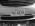
\includegraphics{figures/degradedImg/result-0.png}
	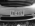
\includegraphics{figures/degradedImg/result-1.png}
	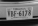
\includegraphics{figures/degradedImg/result-2.png}
	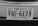
\includegraphics{figures/degradedImg/result-3.png}
	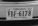
\includegraphics{figures/degradedImg/result-4.png}
	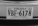
\includegraphics{figures/degradedImg/result-5.png}
	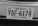
\includegraphics{figures/degradedImg/result-6.png}
	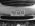
\includegraphics{figures/degradedImg/result-7.png}
	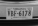
\includegraphics{figures/degradedImg/result-8.png}
	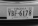
\includegraphics{figures/degradedImg/result-9.png} \\
	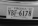
\includegraphics{figures/degradedImg/result-10.png}
	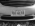
\includegraphics{figures/degradedImg/result-11.png}
	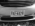
\includegraphics{figures/degradedImg/result-12.png}
	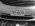
\includegraphics{figures/degradedImg/result-13.png}
	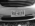
\includegraphics{figures/degradedImg/result-14.png}
	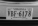
\includegraphics{figures/degradedImg/result-15.png}
	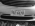
\includegraphics{figures/degradedImg/result-16.png}
	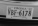
\includegraphics{figures/degradedImg/result-17.png}
	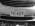
\includegraphics{figures/degradedImg/result-18.png}
	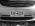
\includegraphics{figures/degradedImg/result-19.png}
	\caption{Conjunto das imagens geradas a partir da imagem de alta resolução. Note a diferença sutil entre as imagens.}
	\label{fig:frames}
\end{figure}

Durante a fase de testes do método, o 
